% =============================================================================
% File      : ex_doc_2-20.tex -- example 2.20
% Author    : Jürgen Hackl <hackl.j@gmx.at>
% Creation  : 2019-08-14
% Time-stamp: <Wed 2019-08-14 17:00 juergen>
%
% Copyright (c) 2019 Jürgen Hackl <hackl.j@gmx.at>
% =============================================================================
\documentclass{standalone}
\usepackage{../../tikz-network}
\begin{document}
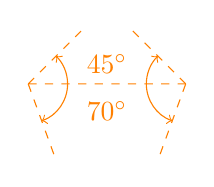
\begin{tikzpicture}
    \Vertex{A}
    \Vertex[x=2]{B}
    \Edge[bend=45](A)(B)
    \Edge[bend=-70](A)(B)
    \draw[orange,dashed](0,0) -- (20mm,0mm)(0,0)--(45:10mm);
    \draw[orange,->] (.5,0) arc (0:45:5mm);
    \draw[orange,dashed](0,0)--(-70:10mm);
    \draw[orange,->] (.5,0) arc (0:-70:5mm);
    \node[orange] (x) at (1,.25) {$45^\circ$};
    \node[orange] (x) at (1,-.35) {$70^\circ$};
    \draw[orange,dashed] (2,0)--++(135:10mm);
    \draw[orange,->] (1.5,0) arc (180:135:5mm);
    \draw[orange,dashed] (2,0)--++(-110:10mm);
    \draw[orange,->] (1.5,0) arc (-180:-110:5mm);
\end{tikzpicture}
\end{document}
% =============================================================================
% eof

%%% Local Variables:
%%% mode: latex
%%% TeX-master: t
%%% End:
